\documentclass[twocolumn]{article}
\usepackage[spanish]{babel}
\usepackage[utf8]{inputenc}
\usepackage{amssymb}
\usepackage{graphicx}
\usepackage{verbatim}
\usepackage{algorithmic}
\usepackage{enumitem}
\usepackage{fancyvrb}
\usepackage{bera}
\setlist{nolistsep}




\author{
Nombre:....................................... \\
    Departamento de Informática y Sistemas \\
    Universidad EAFIT \\
}
\title{
    Estructuras de Datos 2 - ST0247 - 022 \\
    Examen Parcial 2 (lunes)
}
\date{
    Mayo 08, 2017
}

\begin{document}
\vspace{-5cm}
\maketitle


\section*{Criterios de calificación}

\begin{itemize}
\item Selección múltiple con única respuesta
\begin{itemize}
\item Respuesta correcta: 100\%
\item Respuesta incorrecta: 0\%
\end{itemize}

\item Completar código
\begin{itemize}
\item Respuesta correcta 100\%
\item Respuesta incorrecta o vacía 0\% \\
\end{itemize}
\end{itemize}

\textbf{NOTAS IMPORTANTES:}
\begin{itemize}
	\item Responda en la hoja de PREGUNTAS
	\item Marque la hoja de PREGUNTAS
\end{itemize}

\section{Alg. Voraces 20\%}
El problema del \textbf{agente viajero} consiste en responder la siguiente pregunta: Dada
una lista de ciudades y las distancias entre cada par de ciudades, ¿cuál es la
ruta posible más corta que visita a cada ciudad exactamente una vez y regresa a la
ciudad de origen? 

Un algoritmo voraz para solucionar este problem es el \textbf{algoritmo del vecino más
cercano} también llamado el \textbf{Algoritmo de Christofides}. El algoritmo empieza en la primera ciudad y selecciona en
cada iteración una nueva ciudad, no visitada, que sea la más cercana a la inmediamente
anterior. A continuación una implementación del algoritmo del vecino más cercano
que recibe como parámetro un grafo representado como matriz de adyacencia. 

La persona que hizo este código es un ingeniero matemático. En Matlab los índices
empiezan en $1$. Por esta razón, el camino que encuentra el algoritmo empieza con la ciudad numerada con $1$ y trabaja
con ciclos \texttt{while} en lugar de \texttt{for}. Adicionalmente, el programador inicia los índices en $1$, por ejemplo \texttt{i = 1}. Por si fuera poco, 
la variable \texttt{min} no era necesaria inicializarla fuera del bloque \texttt{while} y \texttt{minFlag} hubiera sido
mejor declararla dentro del bloque \texttt{while}. Finalmente,
 el arreglo de visitados sería más eficiente haberlo hecho con tipo \texttt{boolean}. No obstante,
 el programa funciona en Java.

{\small
\begin{verbatim}
01 public void tsp(int adjacencyMatrix[][]) {
02  Stack<Integer> stack = new Stack<Integer>();
03  int numberOfNodes=adjacencyMatrix[1].length-1;
04  int[] visited = new int[numberOfNodes + 1];
05  visited[1] = 1;
06  stack.push(1);
07  int element, dst = 0, i;
08  int min = Integer.MAX_VALUE;
09  boolean minFlag = false;
10  System.out.print(1 + "\t");
11  while (!stack.isEmpty()) {
12   element = stack.peek();
13   i = 1;
14   min = Integer.MAX_VALUE;
15   while (i <= numberOfNodes) {
16    if (adjacencyMatrix[element][i] > 0 
17        && visited[i] == 0) {
18         if (_______> ______) {
19          min = adjacencyMatrix[element][i];
20          dst = i;
21          minFlag = true;
22         }
23    }
24    i++;
25   }
26   if (minFlag) {
27    visited[dst] = 1;
28    stack.push(dst);
29    System.out.print(dst + "\t");
30    minFlag = false;
31    continue;
32   }
33   stack.pop();
34  }
}
\end{verbatim}
}

\texttt{Continue} es una palabra reservada en Java que permite terminar una iteración
de un ciclo abruptamente y pasar a la siguiente iteración del ciclo.\\

1.1  (10\%) Complete el espacio en la línea 18\\


  \_\_\_\_\_\_ $>$ \_\_\_\_\_\_

1.2 (10\%) ¿Cuál es la complejidad asintótica para el peor de los casos?\\


  \_\_\_\_\_\_\_\_\_\_\_\_


%if (min > adjacencyMatrix[element][i])                       {

%O(n^2)


\section{Prog. Dinámica 30\%}

La \textbf{distancia de Levenshtein} es el número mínimo de operaciones requeridas para transformar una cadena de caracteres en otra. Se entiende por operación,  una inserción, eliminación o la sustitución de un carácter. Es útil en programas que determinan cuán similares son dos cadenas de caracteres, como es el caso de los correctores de ortografía. Como un ejemplo, la distancia de Levenshtein entre ``casa'' y ``calle'' es de $3$ porque se necesitan al menos tres operaciones para convertir uno en el otro:

\begin{enumerate}
   \item casa $\rightarrow$ cala (sustitución de 's' por 'l')
  \item  cala $\rightarrow$ calla (inserción de 'l' entre 'l' y 'a')
   \item calla $\rightarrow$ calle (sustitución de 'a' por 'e')
\end{enumerate}

A continuación está una implementación del algoritmo en Java:

{\small
\begin{verbatim}
int minimum(int a, int b, int c) {                            
  return Math.min(Math.min(a, b), c);                                      
}                                                                            
                                                                                
int Levenshtein(String lhs, String rhs) {      
  int[][] distance = new int[lhs.length() + 1]
                            [rhs.length() +1];                                   
  for (int i = 0; i <= lhs.length(); i++)                                 
    distance[i][0] = i;                                                  
  for (int j = 1; j <= rhs.length(); j++)                                 
    distance[0][j] = j;                                                                     
  for (int i = 1; i <= lhs.length(); i++)                                 
    for (int j = 1; j <= rhs.length(); j++)                             
     distance[i][j] = minimum(                                        
      distance[i - 1][j] + 1,                                  
      distance[i][j - 1] + 1,                                  
      distance[i - 1][j - 1] + 
      ((lhs.charAt(i - 1) == rhs.charAt(j - 1)) ? 0 : 1));                                                           
  return distance[lhs.length()][rhs.length()];                          
}                                                                            
\end{verbatim}
}

En Java, el operador incógnita (?) funciona de la siguiente forma: Si \texttt{algo} es verdadero, entonces retorna un \texttt{valor},
de lo contrario retorna otro \texttt{valor}, así:
\texttt{algo? un valor : otro valor}.

2.1 (15 \%) Complete la siguiente tabla, siguiendo el algoritmo de programación dinámica de la distancia de Levenshtein:

\begin{tabular}{| l  | l  | l  | l  | l  | l  | l |}
\hline
  & & c & a & l & l & e \\
 \hline
  & &  &  &  &  &  \\
  \hline
c & &  &  &  &  &  \\
\hline
a & &  &  &  &  &  \\
\hline
s & &  &  &  &  &  \\
\hline
a & &  &  &  &  &  \\
\hline
\end{tabular}

%  	  	c 	a 	l 	l 	e
%   	0 	1 	2 	3 	4 	5
% c 	1 	0 	1 	2 	3 	4
% a 	2 	1 	0 	1 	2 	3
% s 	3 	2 	1 	1 	2 	3
% a 	4 	3 	2 	2 	2 	3

2.2 (15 \%) Complete la siguiente tabla, siguiendo el algoritmo de programación dinámica de la distancia de Levenshtein, para encontrar
la distancia entre madre y mama:

\begin{tabular}{| l  | l  | l  | l  | l  | l  | l |}
\hline
  & & m & a & d & r & e \\
 \hline
  & &  &  &  &  &  \\
  \hline
m & &  &  &  &  &  \\
\hline
a & &  &  &  &  &  \\
\hline
m & &  &  &  &  &  \\
\hline
a & &  &  &  &  &  \\
\hline
\end{tabular}


\section{Algo. voraces 30\%}
El algoritmo de Dijkstra sirve para encontrar el camino más corto
de un vértice a todos los demás de un grafo. A continuación una
implementación en Java.

{\small
\begin{verbatim}
int minVertex (int [] dist, boolean [] v) {
 int x = Integer.MAX_VALUE; //Infinity
 int y = -1;   
 for (int i=0; i<dist.length; i++) 
  if (!v[i] && dist[i]<x) 
     y=i; x=dist[i];
 return y;
}
      
int [] dijsktra(Graph dg, int source) {
  int [] dist = new int [dg.size()]; 
  int [] pred = new int [dg.size()]; 
  boolean [] visited = new boolean [dg.size()]; 
  for (int i=0; i<dist.length; i++) 
    dist[i] = Integer.MAX_VALUE; 
  dist[source] = 0;
  for (int i=0; i<dist.length; i++) {
    int next = minVertex (dist, visited);
    visited[next] = true;
    ArrayList<Integer> n =
        dg.getSuccessors (next); 
    for (int j=0; j<n.size(); j++) {
      int v = n.get(j);
      int d = dist[next] + 
          dg.getWeight(next,v);
      if (dist[v] > d) {
        dist[v] = d;
        pred[v] = next;
      }}}
  return pred;  
}
\end{verbatim}
}

Considere el siguiente grafo:

\begin{center}
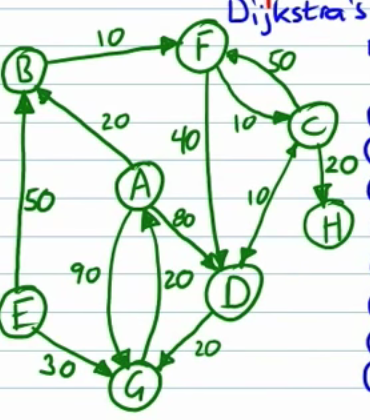
\includegraphics[scale=0.3]{dij.png}
\end{center}

4.1 (20 \%) Complete, por favor, la siguiente tabla, usando
el algoritmo de Dijkstra para encontrar el camino más corto del vértice $A$ a todos los demás. En la tabla, la palabra ``a'' significa ``hasta''.

{\footnotesize
\begin{center}
\begin{tabular}{| c | c | c | c | c | c | c | c | c |}
\hline
Paso  & a & B & C & D & E & F & G & H \\
\hline
1 &  A  & $20$,A  & $\infty$  & $80$, A  & $\infty$   & $\infty$  & $90$, A  & $\infty$  \\
\hline
2 &  B  & $20$,A  &  $\infty$  & $80$, A  & $\infty$  & $30$,B  & $90$,A   & $\infty$  \\
\hline
3 &   &   &   &   &   &   &   &   \\
\hline
4 &   &   &   &   &   &   &   &   \\
\hline
5 &   &   &   &   &   &   &   &   \\
\hline
6 &   &   &   &   &   &   &   &   \\
\hline
7 &   &   &   &   &   &   &   &   \\ 
\hline
8 &   &   &   &   &   &   &   &   \\ 
\hline
\end{tabular}
\end{center}
}

4.2 (10 \%) ¿Cuál es el camino más corto de A a G?

  \_\_\_\_\_\_\_\_\_\_\_\_\_\_\_\_\_\_\_\_


\section{Prog. dinámica 20\%}
%http://www.geeksforgeeks.org/dynamic-programming-set-4-longest-common-subsequence/
El problema de la subsecuencia común más larga es el siguiente. Dadas dos secuencias, encontrar la longitud de la secuencia más larga presente en ambas.
Una subsecuencia es una secuencia que aparece en el mismo orden relativo, pero no necesariamente de forma contigua. Como un ejemplo, ``abc'', ``abg'', ``bdf'',
``aeg'' y ``acefg'' son subsecuencias de ``abcdefg''. Entonces, para una cadena de longitud $n$ existen $2^n$ posibles subsecuencias. Este problema es utilizado
en la implementación del comando \texttt{diff}, para comparación de archivos, disponible en sistemas Unix.  También tiene muchas aplicaciones en bioinformática.

\noindent
Considere los siguientes ejemplos para el problema:
\begin{itemize}
\item Para ``ABCDGH'' y ``AEDFHR'' es ``ADH'' y su longitud es 3.
\item Para ``AGGTAB'' y ``GXTXAYB'' es ``GTAB'' y su longitud es 4.
\end{itemize}

Una forma de resolver este problema es usando \emph{backtracking}, como un ejemplo, para las cadenas  ``AXYT'' y  ``AYZX'', dada una función recursiva \texttt{lcs} 
que resuelve el problema, se obtendría el siguiente árbol (parcial) de recursión:

{\scriptsize
\begin{Verbatim}[commandchars=\\\{\},codes={\catcode`$=3\catcode`_=8}]
                 lcs("AXYT", "AYZX")
                 /                 \textbackslash
    lcs("AXY", "AYZX")            lcs("AXYT", "AYZ")
\_\_\_\_\_\_\_\_\_\_\_\_\_\_\_\_\_\_\_\_\_\_\_\_\_\_\_\_\_\_\_\_\_\_\_\_\_\_\_\_\_\_\_\_\_\_\_\_\_\_\_
    lcs("AXY", "AYZX")          
      /            \textbackslash               
lcs("AX", "AYZX") \textbf{lcs("AXY", "AYZ")}
\_\_\_\_\_\_\_\_\_\_\_\_\_\_\_\_\_\_\_\_\_\_\_\_\_\_\_\_\_\_\_\_\_\_\_\_\_\_\_\_\_\_\_\_\_\_\_\_\_\_\_\_
    lcs("AXYT", "AYZ")
     /             \textbackslash
\textbf{lcs("AXY", "AYZ")} lcs("AXYT", "AY")
\end{Verbatim}
}

Usando backtracking para ese problema, el problema \texttt{lcs(“AXY”, “AYZ”)} se resuelve dos veces. Si dibujamos el árbol de recursión completo, veremos que aparecen más y más problemas repetidos, así como en el caso de serie de Fibonacci. Este problema se puede solucionar guardando la soluciones, que ya se han calculado para los subproblemas, en una tabla; es decir,
usando programación dinámica, como en el algoritmo siguiente:

{\footnotesize
\begin{verbatim}
01 // Precondición: Ambas cadenas x, y son no vacías
02 public static int lcsdyn(String x, String y) {
03  int i,j;
04  int lenx = x.length();
05  int leny = y.length();
06  int[][] table = new int[lenx+1][leny+1];
07 
08  // Inicializa la tabla para guardar los prefijos
09  // Esta inicialización para las cadenas vacías
10  for (i=0; i<=lenx; i++) 
11    table[i][0] = 0;
12  for (i=0; i<=leny; i++)
13    table[0][i] = 0;
14     
15  // Llena cada valor de arriba a abajo
16  // y de izquierda a derecha
17  for (i = 1; i<=lenx; i++) {
18     for (j = 1; j<=leny; j++) {
19        // Si el último caracter es igual
20        if (x.charAt(i-1) == y.charAt(j-1))
21         table[i][j] = 1+table[i-1][j-1];
22        // De lo contrario, tome el máximo
23        else // de los adyacentes
24         table[i][j] = Math.max(table[i][j-1], 
                                  table[i-1][j]);      
25        System.out.print(table[i][j]+" ");
26     }
27     System.out.println();
28   }
29       
30   // Retornar la respuesta (tipo entero, ojo)
31   _______________________________
32   }
\end{verbatim}
}

5.1 (10 \%) ¿Cuál es la complejidad asintótica para el peor de los casos? OJO, $n$ no es una variable en este problema.

  \_\_\_\_\_\_\_\_\_\_\_\_\_\_\_\_\_\_\_\_


5.2 (10 \%) Complete la línea 31

  \_\_\_\_\_\_\_\_\_\_\_\_\_\_\_\_\_\_\_\_

%return table[lenx][leny];
%
%oreturn table[i][j];



\end{document}